\documentclass[12pt]{article}
\usepackage{graphicx} % This lets you include figures
\usepackage{hyperref} % This lets you make links to web locations
\graphicspath{ {./images/} }

\usepackage[rightcaption]{sidecap}
\usepackage{caption}
\usepackage{subcaption}
\usepackage{hyperref}

\usepackage{float}

\usepackage{imakeidx}

\usepackage{tikz}
\usetikzlibrary{shapes.geometric, arrows}
\tikzstyle{startstop} = [rectangle, rounded corners, minimum width=3cm, minimum height=1cm,text centered, draw=black, fill=red!30]
\tikzstyle{io} = [trapezium, trapezium left angle=70, trapezium right angle=110, minimum width=3cm, minimum height=1cm, text centered, draw=black, fill=blue!30]
\tikzstyle{process} = [rectangle, minimum width=3cm, minimum height=1cm, text centered, draw=black, fill=orange!30]
\tikzstyle{decision} = [diamond, minimum width=3cm, minimum height=1cm, text centered, draw=black, fill=green!30]
\tikzstyle{arrow} = [thick,->,>=stealth]

\usepackage{todonotes}

\usepackage{amsmath,amssymb}
\let\amssymbboxplus\boxplus
\let\amssymbboxminus\boxminus

\renewcommand{\boxplus}{\mathbin{\mathop\amssymbboxplus}}
\renewcommand{\boxminus}{\mathbin{\mathop\amssymbboxminus}}

\usepackage[noend]{algpseudocode}


\makeindex


\title{Computer and network security}
\author{Beau De Clercq}
\date{2020-2021}

\begin{document}
	
 \maketitle{}
 
 \tableofcontents
 
 \clearpage
 \newpage
 
 \section{Introduction}
 
 \section{Symmetric ciphers}
 
 \section{Message authentication}
 \subsection{Hash functions}
 A hash function H is a function that takes input data blocks of length M and returns a hash value of fixed size R.\\
 A cryptographic hash function that also satisfies following conditions:
 \begin{itemize}
 	\item One way property: it should be infeasible to find a data object that maps to a predefined hash value.
 	\item Collision free property: it should be infeasible to find 2 data objects that map to the same hash value.
 	\item Use padding to pad up input to fixed length and add the length l of the block in bits. 
 \end{itemize}
By satisfying the first two properties, hash functions can  be used to determine if data has been altered.
\subsubsection{Applications}
Hash functions can be used in an number of applications:
\begin{itemize}
	\item Message authentication: to ensure a message hasn't been altered.
	\item Digital signatures: ensure the authenticity of messages and identity of the sender.
	\item One-way password file: store hash value of password in plain text file.
	\item Intrusion/virus detection: store H(f) for each file to determine if files have been modified.
	\item Pseudorandom function: use H to generate pseudorandom private key.
\end{itemize}
\subsubsection{Security requirements}
Cryptographic hash functions must adhere to following security requirements:
\begin{itemize}
	\item Basic:
	\begin{itemize}
		\item Input data can be of any size
		\item Output is of fixed length
		\item H(x) is easy to compute
	\end{itemize}
	\item Advanced:
	\begin{itemize}
		\item Given h, it is hard to find y: H(y) = h
		\item It is hard to find y: y$\ne$x $\&$ H(y)=H(x)
		\item It is hard to find (x, y): H(x)=H(y)
	\end{itemize}
\end{itemize}

\subsubsection{Attacks}
\begin{itemize}
	\item \underline{Brute force preimage attack}\\
	The goal of this attack is to find a y such that H(y) = h for a given hash value h.\\
	The attack itself goes as follows:\\
	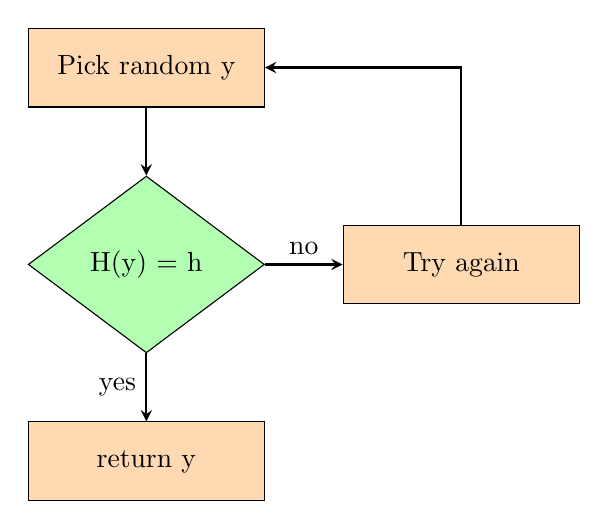
\begin{tikzpicture}[node distance=2cm]
	
	\node (pro1) [process] {Pick random y};
	\node (dec1) [decision, below of=pro1, yshift=-0.5cm] {H(y) = h};
	\node (pro2a) [process, below of=dec1, yshift=-0.5cm] {return y};
	\node (pro2b) [process, right of=dec1, xshift=2cm] {Try again};

	\draw [arrow] (pro1) -- (dec1);
	\draw [arrow] (dec1) -- node[anchor=east] {yes} (pro2a);
	\draw [arrow] (dec1) -- node[anchor=south] {no} (pro2b);
	\draw [arrow] (pro2b) |- (pro1);

	\end{tikzpicture}\\
	On average this attack need $2^{m-1}$ attempts for an m-bit hash value.
	\item \underline{Brute force collision resistance attack}\\
	The goal of this attack is to find two values x and y such that H(x) = H(y). This attack need $2^{\frac{m}{2}}$ attempts for an m-bit hash value.\\
	\todo[inline]{Add image of attack from slides}
\end{itemize}
 
 \subsection{Secure Hash Algorithm (SHA)}
 \todo[inline]{Add SHA overview from slides}
 \subsubsection{SHA512}
 \todo[inline]{Add image from slides}
 \subsubsection{SHA512 block processing}
 \todo[inline]{Add image from slides}
 \todo[inline]{Add image of round function from slides}
 In this 80 round process, a message of 1024 bits is transformed into 80 values of 64 bits each which are then individually processed in sequence by means of a round function.\\
 After the final round a word-by-word addition 64-bit words mod$2^{64}$ is performed to obtain the final hashed value.
 \subsubsection{Message schedule}
 The first 16 words $W_0 .. W_{15}$ are derived directly from the input block $M_i$. All other words are derived as follows:
 \begin{align*}
 	W_t = W_{t-16} \boxplus \delta_0(W_{t-15}) \boxplus W_{t-7} \boxplus \delta_1(W_{t-2})\\
 	\delta_0(x) = ROTR^1(x) \oplus ROTR^8(x) \oplus SHR^7(x)\\
 	\delta_1(x) = ROTR^{19}(x) \oplus ROTR^{61}(x) \oplus SHR^6(x)\\
 	ROTR^n(x) = \text{circular right bit-shift by n bits}\\
 	SHR^n(x) = \text{right bit-shift of x by n bits with}\\
 	 \text{padding by n zeros on the left}
 \end{align*}
 
 \subsection{Length extension attack and SHA3}
 \subsubsection{Length extension attack}
 Type of attack where an attacker can use H($M_1$) and the length of $M_1$ to calculate H($M_1|M_2$) for an attack controlled message $M_2$ without needing to know the content of $M_1$. This is done by taking the old message and using it as 'intermediary' input in the hashing algorithm.
 \subsubsection{SHA3}
 \todo[inline]{Add image from slides}
 
 \subsection{Message authentication}
 There are 8 types of attacks:
 \begin{enumerate}
 	\begin{multicols}{2}
 		\item Disclosure of message content
 		\item Traffic analysis
 		\item Masquerade
 		\item Content modification
 		\item Sequence modification
 		\item Timing modification
 		\item Source repudiation
 		\item Destination repudiation
 	\end{multicols}
 \end{enumerate}
 Items 1 and 2 can be countered using confidentiality mechanisms, eg symmetric encryption.\\
 Items 3 to 6 can be countered by using \underline{message authentication} to verify that the received message hasn't been altered.\\
 \underline{Digital signatures} can be seen as an extension to message authentication as it is an authentication technique that also includes measures to counter repudiation by the source.\\
 \newline
 A message authentication function is a function that produces an authenticator (a value to be used to authenticate a message). There are 3 classes of message authentication functions:
 \begin{itemize}
 	\item Hash functions:
 	\begin{itemize}
 		\item Concatenate message M with secret key S and hash the stream
 		\item Send message M together with hash value: if it is intercepted an attacker can't create a new hash value since the key is unknown
 		\item Check authentication: combine M with S, hash the stream and compare with received hash value
 	\end{itemize}
 	\item Message encryption, eg using symmetric encryption, provides both confidentiality and authentication if key K is secret. If the decrypted message M is not meaningful then the message can be considered altered.
 	\item Message authentication code (MAC): generates fixed-size cryptographic checksum based on message and secret key
 	\begin{itemize}
 		\item Does not need to be reversible
 		\item send message with checksum: if the checksum calculated by the receiver doesn't match then the message has been altered
 		\item Cannot be used to provide digital signatures: a signature need to be verifiable by anyone and MAC requires the use of a secret key
 	\end{itemize}
 \end{itemize}
 \subsubsection{Security requirements for MAC}
 \begin{itemize}
 	\item If an opponent observes $M$ and $MAC(K, M)$, it should be infeasable to construct $M'$ such that $MAC(K, M') == MAC(K, M)$.
 	\item Given 2 randomly chosen messages $M$ and $M'$, the probability that $MAC(K, M) == MAC(K, M')$ should be $2^{-N}$ for an N-bit code. $-->$ codes should be distributed uniformly and random over the entire output space
 	\item If $M'$ is a known transformation of $M$, then $\mathbb{P}(MAC(K, M) = MAC(K, M') = 2^{-N}$.
 \end{itemize}

 \subsection{Message authentication codes}
 \subsubsection{Cipher-based MAC (CMAC)}
 \begin{itemize}
 	\item $M$ is split into fixed size blocks $M_1, ..., M_N$.
 	\item $M_1$ is encrypted with key $K$ of k bits.
 	\item Resulting block is then XORed with next input block, the result is then encrypted with the same key $K$. This process is repeated until block $M_{N-1}$.
 	\item At the final block $M_N$: XOR $M_N$ with $M_{N-1}$ and b-bit constant $K_1$ derived from the original key.
 	\item Encrypt the result using key $K$, then the leftmost significant bits represent the tag.
 	\item If $M$ is not a multiple of b: last block is padded with $10..0$ and $K_2$ is used in stead of $K_1$.
 	\item Determining $K_1$ and $K_2$: 
 	\begin{equation*}
 		L = E(K, 0^b), K_1 = L*x, K_2 = L*x^2 
 	\end{equation*}
 	where multiplication happens in $GF(2^b)$
 \end{itemize}
 
 \subsubsection{Hash-based MAC (HMAC)}
 \begin{itemize}
 	\item Advantages: hash functions execute faster and library code is widely available.
 	\item Main issue: a secret key needs to be used when using a hash function.
 	\item Objectives:
 	\begin{itemize}
 		\item To use, without modification, available hash functions;
 		\item To allow for easy replaceability of the hash function;
 		\item To preserve the hash function's original performance;
 		\item To use and handle keys in a simple way;
 		\item To have a well understood cryptographic analysis.
 	\end{itemize}
 	\item Structure: \todo[inline]{copy image from slide}
 	\item Cryptographic strengths:
 	\begin{itemize}
 		\item HMAC can be proven secure provided that the embedded hash function has some reasonable cryptographic strengths.
 		\item A successful attack on HMAC is equivalent to one of the following:
 		\begin{itemize}
 			\item The attacker is able to compute an output of the compression function.
 			\item The attacker finds collisions in the hash function.
 		\end{itemize}
 	\end{itemize}
 \end{itemize}

 
 \section{Asymmetric encryption}
 \subsection{Introduction}
 Asymmetric encryption uses both a public and private key, it's working is based on mathematical functions rather than substitution and permutations.\\
 AE addresses two concerns with symmetric encryption:
 \begin{itemize}
 	\item Secret keys are distributed using a trusted key distribution center
 	\item It does not enable digital signatures
 \end{itemize}
 \subsubsection{Confidentiality using AE}
 Assume there is some source A that produces a message in plaintext X which is intended for destination B. B generates a related pair of keys: a public key, $PU_b$, and a private key, $PR_b$. $PR_b$ is known only to B, whereas $PU_b$ is publicly available and therefore accessible by A.\\ With the message X and the encryption key $PU_b$ as input, A forms the ciphertext $Y = E(PU_b, X)$. The intended receiver, in possession of the matching private key, is able to invert the transformation: $X = D(PR_b,Y)$.\\ 
 An adversary, observing Y and having access to $PU_b$, but not having access to $PR_b$ or X, must attempt to recover X and/or $PR_b$. It is assumed that the adversary does have knowledge  of  the  encryption  (E)  and decryption  (D) algorithms.  If  the adversary is interested only in this particular message, then the focus of effort is to recover X by generating a plaintext estimate $\widehat{X}$. Often, however, the adversary is interested in being able to read future messages as well, in which case an attempt is made to recover $PR_b$ by generating an estimate $\widehat{PR_b}$.
 
 \subsubsection{Authentication using AE}
 In this case, A prepares a message to B and encrypts it using A’s private key before transmitting it. B can decrypt the message using A’s public key. Because the message was encrypted using A’s private key, only A could have prepared the message.Therefore,the entire encrypted message serves as a digital signature. In addition, it is impossible to alter the message without access to A’s private key, so the message is authenticated both in terms of source and in terms of data integrity.\\
 In this scheme, the entire message is encrypted, which, although validating both author and contents, requires a great deal of storage. Each document must be kept in plaintext to be used for practical purposes. A copy also must be stored in ciphertext so that the origin and contents can be verified in case of a dispute. A more efficient way of achieving the same results is to encrypt a small block of bits that is a function of the document. Such a block, called an \underline{authenticator}, must have the property that it is infeasible to change the document without changing the authenticator. If the authenticator is encrypted with the sender’s private key, it serves as a signature that verifies origin, content, and sequencing.
 
 \subsubsection{Combining confidentiality and authentication}
 It is possible to provide both the authentication function and confidentiality by a double use of the public-key scheme
 \begin{itemize}
 	\item $Z = E(PU_b,E(PR_a,X))$
 	\item $X = D(PU_a,D(PR_b,Z))$
 \end{itemize} 
 where $(PU_a, PR_a)$ is a key pair generated by the sender and is used for authentication and $(PU_b, PR_b)$ is a key pair generated by the receiver and is used for confidentiality.\\
 Encryption of a message $M$ then goes as follows: $M \rightarrow E(M, PR_a) \rightarrow E(E(M, PR_a), PU_b) \rightarrow C$.\\
 Decryption of a ciphertext $C$ happens as follows: $C \rightarrow D(C, PR_b) \rightarrow D(D(C, PR_b), PU_a) \rightarrow M$.
 
 \subsubsection{Requirements for public-key cryptography}
 \begin{itemize}
 	\begin{multicols}{2}
 		\item It is computationally easy to generate the key pair $(PU_b, PR_b)$.
 		\item It is computationally easy, given the public key $PU_b$ and a message $M$, to generate the corresponding ciphertext $C = E(PU_b, M)$.
 		\item It is computationally easy, given the private key $PR_b$ and a ciphertext $C$, to recover the plaintext $M = D(PR_b, C) = D(PR_b, E(PU_b, M))$.
 		\item It is computationally infeasible, knowing $PU_b$ or $PR_b$, to generate the other key.
 		\item It is computationally infeasible, knowing $PU_b$ and ciphertext $C$, to recover the original message $M$.
 		\item Optional: the two keys can be applied in any order.
 	\end{multicols}
 \end{itemize}
 
 \subsection{Rivest-Shamir-Adleman (RSA)}
 \subsubsection{RSA basics}
 In RSA, each plaintext block $M$ is represented by a number smaller than $n$, resulting in a block size of at most $^2log(n)+1$ bits. In practice a block size of $i$ bits is used with $2^i\leq n\leq 2^{i+1}$.\\
 Encryption and decryption happen according to following formulas:
 \begin{itemize}
 	\item Encryption: $C = M^e \text{ mod }n$
 	\item Decryption: $M = C^d \text{ mod }n = M^{ed} \text{ mod } n$
 \end{itemize}
Since both sender and receiver know $n$, only the sender knows $e$ and $d$ is known only to the receiver, the public key $PU$ en private key $PB$ become
\begin{itemize}
	\item $PU = \{e, n\}$
	\item $PB = \{d, n\}$
\end{itemize}
\textbf{Finding suitable values for $e, d$ and $n$}\\
Assuming $M$ and $n$ are relative prime, Euler's theorem states 
\begin{equation*}
M^{\phi(n)+1} \equiv M \text{ mod } n = M^{ed} \text{ mod } n \Leftrightarrow ed \equiv 1 \text{ mod }\phi(n) \Leftrightarrow d \equiv e^{-1}\text{ mod }\phi(n)
\end{equation*}
where $\phi(n)$ is the Euler totient function that returns the number of integers $k (1\leq k\leq n)$ for which $gcd(n, k) = 1$.\\
\textbf{How to guarantee $M$ and $n$ relative prime}\\
If $n = pq$ with $p$ and $q$ prime, then $M$ and $n$ are relative prime if $M$ is different from $1, p$ and $q \Rightarrow \phi(n) = (p-1)(q-1) (\Rightarrow ed\text{ mod }\phi(n) = 1)$.
 \subsubsection{RSA ingredients}
  \begin{itemize}
 	\begin{multicols}{2}
 		\item Two prime numbers $p$ and $q$, chosen privately
 		\item Integer $n = pq$, calculated and publicly available
 		\item Value $e$ chosen by key generator with $gcd(\phi(n), e) = 1; 1<e<\phi(n)$ publicly available
 		\item Value $d \equiv e^{-1}\text{ mod }\phi(n)$ calculated and private 
 	\end{multicols}
 \end{itemize}
Note that it should be infeasible to calculate $p, q$ and that this is the case if $n$ is large enough.
 
 \subsection{Efficient RSA operations}
 \subsubsection{Efficient exponentiation in modular arithmetic}
 To avoid integer overflow during calculations, we can use the property that $[(a\text{ mod }n)(b\text{ mod }n)]\text{ mod }n = (ab)\text{ mod }n$. Similarly we can make calculating large exponents more efficient by reusing intermediary results, eg $x^{13} = x*x^4*x^8$. We can calculate $x\text{ mod }n$, $x^2\text{ mod }n$, $x^4\text{ mod }n$ and $x^8\text{ mod }n$ where each reuses the previous result.\\
 $\Rightarrow$ \textbf{Algorithm to find $a^b\text{ mod }n$}\\
 $b$ can be expressed as a binary number $b_kb_{k-1}...b_1b_0$, or $b = \Sigma_{b_i\ne 0}2^i$, therefore $a^b = a^{\Sigma_{b_i\ne 0}2^i} = \Pi_{b_i\ne 0}a^{2^i}$.\\
 $\Rightarrow a^b\text{ mod }n = [\Pi_{b_i\ne 0}a^{2^i}]\text{ mod }n = [\Pi_{b_i\ne 0}a^{2^i}\text{ mod }n]\text{ mod }n $\\
 $\Rightarrow$Algorithm:
 \begin{algorithmic}
 	\State $f = 1$
 	\For {$i=k$ down to $0$}
 	\State $f = (ff)\text{ mod }n$
 	\If {$b_i = 1$}
 	\State $f = (fa)\text{ mod }n$
 	\EndIf
	\EndFor
	\State return $f$
 \end{algorithmic}
 	
 \subsubsection{Efficient operation using public key}
 To make encryption as efficient as possible, chose an exponent with few 1 bits $\rightarrow$ the most common choice is $2^{16+1}, 3, 17$ since each of these numbers only has 2 1 bits. Note that small values are vulnerable to simple attacks but that this can be solved by adding a unique psuedorandom bit string as padding.
 
 \subsubsection{Efficient operation using private key}
 If $e$ is chosen to be small, then $d$ is large by definition. To speed up calculations for large $d$ we can use the Chinese remainder theorem.\\
 We need to compute $M = C^d\text{ mod }n$. Now define $V_p = C^d\text{ mod }p$ and $V_q = C^d\text{ mod }q$. Applying the CRT gives $M = (V_pX_p + V_qX_q)\text{ mod }n$ with $X_p = q(q^{-1}\text{ mod }p)$ and $X_q = p(p^{-1}\text{ mod }q)$.\\
 Using Fermat's theorem we get that $V_p = C^{d\text{ mod }(p-1)}\text{ mod }p$ and $V_q = C^{d\text{ mod }(q-1)}\text{ mod }q$ where both $d\text{ mod }(p-1)$ and $d\text{ mod }(q-1)$ can be pre-calculated since $p, q$ and $d$ are known in advance.\\
 By doing this precalculation, calculation of $M$ is about 4 times more efficient.
 
 \subsubsection{Efficient key generation}
 \begin{enumerate}
 	\item Determine 2 prime numbers $p$ and $q$.\\
 	Any adversary will know $n=pq$, so in order to prevent brute force attacks $p$ and $q$ should be large enough and the method to find large $p$ and $q$ should be efficient.\\
 	$\rightarrow$ Generate a random uneven number with the desired order of magnitude. If the number is determined to be prime, then return it. Else we generate a new number and repeat the process.
 	\item Select $e$ or $d$ and calculate the other.\\
 	If $p$ and $q$ are found, than $n$ is found and $\phi(n) = (p-1)(q-1)$ is found. Now lets select $e$ such that $gcd(\phi(n), e) = 1$ and calculate $d$ such that $d\equiv e^{-1}(\text{ mod }\phi(n))$. Both values can be calculated simultaneously using the Extended Euclids Algorithm. \\
 	One possible strategy is to select random numbers $e$ until one is relative prime to $\phi(n)$.
 \end{enumerate}
 
 \subsection{Attacks against RSA}
 \subsubsection{Brute force attacks}
 Try all possible private keys $(d, n)$. RSA is safe if $n$ is chosen large enough: minimum 3072 bits for $n$ with RSA, in symmetric encryption 128 suffice.
 
 \subsubsection{Mathematical attacks}
 Factor the product of $p$ and $q$ given $n$. There are 3 approaches to this kind of attack.
 \begin{enumerate}
 	\item Factor $n$ into 2 primes $p$ and $q$
 	\item Determine $\phi(n)$ directly without finding $p$ and $q$
 	\item Determine $d$ directly without finding $\phi(n)$
 \end{enumerate}
The first two options are mathematically equivalent and easier than the last option.\\
This gives rise to 2 threats to the use of large key sizes:
\begin{itemize}
	\item Continuously improving computational power
	\item Refinement of factoring algorithms
\end{itemize}
There are a few safety precautions that can be taken:
\begin{itemize}
	\item $p$ and $q$ should be nearly the same number of digits
	\item Both $(p-1)$ and $(q-1)$ should contain a large prime factor
	\item $gcd(p-1, q-1)$ should be small
\end{itemize}

 \subsubsection{Timing attacks}
 Exploit the running time of decryption algorithm. This is a ciphertext only attack where a snooper can determine the private key by keeping track of how long it takes to decipher the message. It is applicable to all public key encryption algorithms and for RSA, it uses the timings of the modular exponentiation algorithm. Counter measures include constant exponentiation time (which leads to degraded performance), adding a random delay or by using the blinding technique.\\
 In the blinding technique the operation $M=C^d\text{ mod }n$ is replaced by
 \begin{enumerate}
 	\item Generate a random number $r \in ]0, n-1]$
 	\item Compute $C' =Cr^e \text{ mod }n$ where $e$ is the public exponent
 	\item Compute $M' = (C')^d \text{ mod } n$
 	\item Compute $M = M'r^{-1}$ 
 \end{enumerate}
 This method results in a 2-10\% performance loss.
 
 \subsubsection{Chosen ciphertext attacks}
 Exploit properties of RSA. In this attack the attacker chooses some ciphertext and is given the corresponding plaintext in return. Another possibility is that the attacker sends chosen blocks of data that yield additional information useful for cryptoanalysis.\\
 Given the property that $E(PU,M_1)xE(PU,M_2) = E(PU, M_1xM_2)$ and $C=M^e\text{ mod }n$, we can derive $M$ using the CCA attack as follows
 \begin{itemize}
 	\item Compute $x = (Cx2^e)\text{ mod }n$
 	\item Submit $x$ as a chosen ciphertext and receive $y = x^d\text{ mod }n$
 \end{itemize}
$\Rightarrow x = (C\text{ mod }n)x(2^e\text{ mod }n) = (M^e\text{ mod }n)x(2^e\text{ mod }n) = (2M)^e\text{ mod }n$\\
Therefore $y = (2M)\text{ mod }n$, from which $M$ can be easily deduced.
 
 \subsection{Digital signatures}
 \subsubsection{Introduction}
 \includegraphics[width=\linewidth]{./slides/L4P5intro.PNG}\\
 Authentication vs signatures:
 \begin{itemize}
 	\item Authentication: protects against third parties, only use single private key which is securely shared between sender and receiver $\rightarrow$ verify content of message was not altered.
 	\item Signatures: provides additional securities, ensures that anyone can verify that the message was indeed sent by the sender.
 \end{itemize}
 \subsubsection{Required properties of a digital signature}
 A digital signature must:
 \begin{enumerate}
 	\item Verify the author and time of the signature $\rightarrow$ avoid misuse of private key
 	\item Authenticate the contents at the time of the signature
 	\item Be verifiable by third parties to resolve disputes $\rightarrow$ cannot be provided by MAC
 \end{enumerate}
 
 \subsubsection{RSA-PSS}
 \includegraphics[width=\linewidth]{./slides/L4P5RSAPSS.PNG}\\
 We discuss the RSA Probabilistic Signature Scheme (RSA-PSS), which is the latest of  the RSA schemes and the one that RSA Laboratories recommends as the most secure of the RSA schemes.\\
 We show how the signature is formed by a signer with private key $\{d, n\}$ and public key $\{e, n\}$. Treat the octet string $EM$ as an unsigned, nonnegative binary integer $m$. The signature $s$ is formed by encrypting $m$ as follows: $s = m^d \text{mod} n$.\\
 Let $k$ be the length in octets of the RSA modulus $n$. For example if the key size for RSA is 2048 bits, then $k$ = 2048/8 = 256. Then convert the signature value $s$ into the octet string $S$ of length $k$ octets.\\
 \includegraphics[width=\linewidth]{./slides/L4P5RSAPSSENC.png}\\
 The first stage in generating an RSA-PSS signature of a message $M$ is to generate from $M$ a fixed-length message digest, called an encoded message. We define the following parameters and functions:
 \begin{itemize}
 	\item  Options
 	\begin{itemize}
 		\item Hash: hash function with output hLen octets. The current preferred alternative is SHA-1, which produces a 20-octet hash value.
 		\item MGF: mask generation function. The current specification calls for MGF1.
 		\item $sLen$: length in octets of the salt. Typically sLen = hLen, which for the
 		current version is 20 octets.
 	\end{itemize}
 	\item Input
 	\begin{itemize}
 		\item $M$: message to be encoded for signing.
 		\item $emBits$: This value is one less than the length in bits of the RSA modulus n.
 	\end{itemize}
 	\item Output
 	\begin{itemize}
 		\item EM: encoded message. This is the message digest that will be encrypted to form the digital signature.
 	\end{itemize}
 	\item Parameters
 	\begin{itemize}
 		\item $emLen$: length of EM in octets = $emBits/8$.
 		\item padding1: hexadecimal string 00 00 00 00 00 00 00 00; that is, a string of 64 zero bits.
 		\item padding2 : hexadecimal string of 00 octets with a length (emLen - sLen - hLen - 2) octets, followed by the hexadecimal octet with 63 (emLen - sLen - hLen - 2) octets, followed by the hexadecimal octet with value 01.
 		\item salt: a pseudorandom number.
 		\item bc: the hexadecimal value BC.
 	\end{itemize}
 \end{itemize}
The encoding process consists of the following steps.
\begin{itemize}
	\item Generate the hash value of M: $mHash = Hash(M)$
	\item Generate a pseudorandom octet string salt and form block $M' = padding1 || mHash || salt$
	\item Generate the hash value of M': $H = Hash(M')$
	\item Form data block $DB = padding2 || salt$
	\item Calculate the $MGF$ value of H: $dbMask = MGF(H, emLen - hLen - 1)$
	\item Calculate $maskedDB = DB \bigoplus dbMsk$
	\item Set the leftmost 8 $emLen - emBits$ bits of the leftmost octet in $maskedDB$ to 0
	\item $EM = maskedDB || H || 0xbc$
\end{itemize}

 \subsubsection{RSA-PSS MGF (Mask Generating Function)}
 The goal is to generate a cryptographically secure variable length $L$ hash code using a fixed length output cryptographic hash function $H$, eg SHA.\\
 \includegraphics[width=0.8\linewidth]{./slides/L4P5RSAPSSMGF.PNG}
 
 \subsubsection{RSA-PSS signature verification}
  \includegraphics[width=0.8\linewidth]{./slides/L4P5RSAPSSSIGVER.PNG}\\
  For signature verification, treat the signature $S$ as an unsigned, nonnegative binary integer $s$. The message digest $m$ is recovered by decrypting $s$ as follows: $m = se \text{ mod } n$.\\
  Then, convert the message representative $m$ to an encoded message $EM$ of length $emLen = modBits -\frac{1}{8}$ octets, where $modBits$ is the length in bits of the RSA modulus $n$.
 
 \section{Key distribution}
 \subsection{Symmetric private key distribution}
 \noindent\fbox{%
 	\parbox{\textwidth}{%
 		How to share a private key between 2 parties without others having access to it?
 	}%
 }

 There are a few different distribution methods for parties $A$ and $B$:
 \begin{enumerate}
 	\item $A$ selects the key and physically delivers it to $B$
 	\item Third party selects a key and physically delivers it to $A$ and $B$
 	\item If $A$ and $B$ already share a key, a new key can be encrypted using the old key and transmitted over the network
 	\item If $A$ and $B$ have anencrypted connection to a third party $C$, $C$ can deliver a key on the encrypted link to $A$ and $B$
 \end{enumerate}
 Solutions 1 and 2 are infeasible in large scale networks. If in solution 3 an attacker determines a single key then all future keys are compromised, due to the amount of keys that need to be maintained this solution too can only be used on small scale.\\
 It thus follows that solution 4 is the preferred one.

 \subsubsection{Decentralized key control without third party}
 This way of working avoids the need for a central trusted authority, but it can only be used in small scale scenarios like local networks.\\
 \includegraphics[width=\linewidth]{./slides/L5P1.PNG}
 \begin{enumerate}
 	\item $A$ send $ID_A||N_1$ to $B$ where $N_1$ is a random nonce
 	\item $B$ uses the previously shared master key $K_m$ to encrypt a newly generated key $K_s$
 	\item After decryption $A$ will send $E(K_s, f(N_2))$ to $B$
 \end{enumerate}
This approach uses $\frac{N(N-1)}{2}$ keys in a network with $N$ hosts.
 
 \subsection{Key Distribution Centers (KDCs)}
 \noindent\fbox{%
 	\parbox{\textwidth}{%
 		Centralized authority that distributes keys using symmetric encryption.
 	}%
 }

 \subsubsection{Hierarchical structure}
 Keys are stored on 2 levels:
 \begin{itemize}
 	\item Session keys: temporary keys used between two end systems, discarded after logical session ends.
 	\item Master keys: used to safely encrypt and transmit session keys $\rightarrow$ maintained between KDC and hosts, only used when host requests new session key.
 \end{itemize}

 \subsubsection{KDC scenario}
 \includegraphics[width=\linewidth]{./slides/L5P2KDC.PNG}
 
 \subsubsection{Hierarchical key control}
 A hierarchy of KDCs manages different parts of an internetwork where each local KDC distributes keys in the local network.\\
 Higher layer KDCs can coordinate key distribution across networks.
 
 \subsubsection{Transparent key control scheme}
 For providing end-to-end encryption in connection-oriented protocols.
 \begin{enumerate}
 	\item Host sends packet to request connection
 	\item Security service buffers packet; asks KDC for session key
 	\item KDC distributes session key to both hosts
 	\item Buffered packet is transmitted
 \end{enumerate}
 
 \subsection{Asymmetric private key distribution}
 \subsubsection{Symmetric key distribution using asymmetric encryption}
 \includegraphics[width=\linewidth]{./slides/L5P3SYM.PNG}\\
 This scheme is vulnerable to "man-in-the-middle" attacks $\rightarrow$ same scheme but with an attacker in the middle\footnote{Duh}.
 
 \subsubsection{Diffie-Hellman key exchange}
 Enables 2 users to securely exchange a key (eg for use in subsequent symmetric encryption).\\
 It is based on the difficulty to calculate discrete logarithms. The exponent $i$ is the discrete logarithm of $b$ for base $a$ mod $p$: $d\text{ log}_{a,p}(b)=i \Leftrightarrow b\equiv a^i\text{ mod }p$.\\
 Parties share the publicly known pair $(q,\alpha)$ where $q$ is a prime number and $\alpha$ is an integer and prime root of $q$, meaning a unique exponent $i$ exists for every integer $b<q$ such that $b\equiv\alpha^i\text{ mod }q$.\\
 Private keys are random number $X_A$ and $X_B$ both smaller than $q$. The public keys are $Y_A = \alpha^{X_A}\text{ mod }q$ and $Y_B = \alpha^{X_B}\text{ mod }q$. The shared secret key $K = (Y_B)^{X_A}\text{ mod }q = (Y_A)^{X_B}\text{ mod }q$ can be calculated.\\
 To an attacker, $q, \alpha, Y_A$ and $Y_B$ are available. This means that the private key of $B$ can be calculated as $X_B=d\text{ log}_{\alpha, q}(Y_B)$. The security of Diffie-Hellman lies in the fact that it is easy to calculate exponentials modulo a prime number but that it is hard to calculate discrete logarithms.\\
 The "man-in-the-middle" attack is still possible.
 
 \subsection{Secure distribution of public keys}
 There are 4 general techniques for public key distribution:
 \begin{enumerate}
 	\item Public announcement: broadcast public keys to anyone
 	\item Public directory: dynamic centralized directory of keys
 	\item Public key authority: tightly controlled central directory
 	\item Public key certificates: decentralized secure key exchange
 \end{enumerate}
Both (1) and (2) are not safe, (3) has scalability issues due to the central nature. Hence, (4) is the preferred solution due to better scalability.
 
 \subsubsection{Public announcement}
 Since there is no form of control, anyone can forge an announcement and pretend to be $A$, spreading their own public key.
 
 \subsubsection{Public directory}
 Keys are registered in person or using secure authenticated communication. If the directory's private key is stolen, an attacker can counterfeit public keys.
 
 \subsubsection{Public key authority}
 \includegraphics[width=\linewidth]{./slides/L5P4PKA.PNG}
 
 \subsubsection{Certificates} 
 Central authority only used to generate a certificate that consists of the public key, the ID of the owner the trusted third party's signature. A certificate must adhere to following requirements:
 \begin{itemize}
 	\item Any participant can determine the name and public key of the owner
 	\item Any participant can verify that the certificate originated from the certificate authority and is not counterfeit
 	\item Only the certificate authority can create and update certificates
 	\item Any participant can verify the time validity of the certificate
 \end{itemize}
\includegraphics[width=0.8\linewidth]{./slides/L5P4CERT.PNG}
 
 \subsection{X.509 certificates}
 
 \subsubsection{Certificate generation/working}
 \includegraphics[width=\linewidth]{./slides/L5P5WORK.PNG}
 
 \subsubsection{X.509 format}
 \includegraphics[width=\linewidth]{./slides/L5P5FORM.PNG}
 
 \subsubsection{CA organization}
 
 If the user community is large, eg the internet, then multiple CA's are needed.\\
 \noindent\fbox{%
 	\parbox{\textwidth}{%
 		$Y<<X>>$: certificate of user $X$ is issued by CA $Y$.
 	}%
 }
 \begin{figure}[H]
 	\begin{subfigure}{.7\textwidth}
 		\includegraphics[width=.8\linewidth]{./slides/L5P5ORG1.PNG}
 	\end{subfigure}%
 	\begin{subfigure}{.7\textwidth}
 		\includegraphics[width=.8\linewidth]{./slides/L5P5ORG2.PNG}
 	\end{subfigure}
 \end{figure}
 
 \subsubsection{Certificate revocation}
 
\begin{multicols}{2}
	Revocation may be needed if:
	\begin{itemize}
		\item User's private key is possibly compromised
		\item User is no longer certified by CA
		\item CA's certificate is possibly compromised
	\end{itemize}
	Each CA maintains a CRL (certificate revocation list) with all non-expired but revoked certificates. \\
	\includegraphics[width=\linewidth]{./slides/L5P5CRL.PNG}
\end{multicols}

 
 \subsubsection{Certificate extensions field}
 \includegraphics[width=\linewidth]{./slides/L5P5EXT.PNG}
 
 \subsubsection{Public Key Infrastructure (PKI)}
 Set of hardware, software, people, policies and procedures needed to create, manage, store, distribute and revoke digital certificates based on asymmetric cryptography.\\
 PKI objective: enable secure, convenient and efficient acquisition of public keys.\\
 $\rightarrow$ PKI X.509: formal, generic model based on X.509 to deploy certificate-based architecture on the internet.\\
 \includegraphics[width=\linewidth]{./slides/L5P5PKIMOD.PNG}\\
 \includegraphics[width=\linewidth]{./slides/L5P5PKIMAN.PNG}
  
\end{document}







